%% bare_conf.tex
%% V1.4
%% 2012/12/27
%% by Michael Shell
%% See:
%% http://www.michaelshell.org/
%% for current contact information.
%%
%% This is a skeleton file demonstrating the use of IEEEtran.cls
%% (requires IEEEtran.cls version 1.8 or later) with an IEEE conference paper.
%%
%% Support sites:
%% http://www.michaelshell.org/tex/ieeetran/
%% http://www.ctan.org/tex-archive/macros/latex/contrib/IEEEtran/
%% and
%% http://www.ieee.org/

%%*************************************************************************
%% Legal Notice:
%% This code is offered as-is without any warranty either expressed or
%% implied; without even the implied warranty of MERCHANTABILITY or
%% FITNESS FOR A PARTICULAR PURPOSE! 
%% User assumes all risk.
%% In no event shall IEEE or any contributor to this code be liable for
%% any damages or losses, including, but not limited to, incidental,
%% consequential, or any other damages, resulting from the use or misuse
%% of any information contained here.
%%
%% All comments are the opinions of their respective authors and are not
%% necessarily endorsed by the IEEE.
%%
%% This work is distributed under the LaTeX Project Public License (LPPL)
%% ( http://www.latex-project.org/ ) version 1.3, and may be freely used,
%% distributed and modified. A copy of the LPPL, version 1.3, is included
%% in the base LaTeX documentation of all distributions of LaTeX released
%% 2003/12/01 or later.
%% Retain all contribution notices and credits.
%% ** Modified files should be clearly indicated as such, including  **
%% ** renaming them and changing author support contact information. **
%%
%% File list of work: IEEEtran.cls, IEEEtran_HOWTO.pdf, bare_adv.tex,
%%                    bare_conf.tex, bare_jrnl.tex, bare_jrnl_compsoc.tex,
%%                    bare_jrnl_transmag.tex
%%*************************************************************************

% *** Authors should verify (and, if needed, correct) their LaTeX system  ***
% *** with the testflow diagnostic prior to trusting their LaTeX platform ***
% *** with production work. IEEE's font choices can trigger bugs that do  ***
% *** not appear when using other class files.                            ***
% The testflow support page is at:
% http://www.michaelshell.org/tex/testflow/



% Note that the a4paper option is mainly intended so that authors in
% countries using A4 can easily print to A4 and see how their papers will
% look in print - the typesetting of the document will not typically be
% affected with changes in paper size (but the bottom and side margins will).
% Use the testflow package mentioned above to verify correct handling of
% both paper sizes by the user's LaTeX system.
%
% Also note that the "draftcls" or "draftclsnofoot", not "draft", option
% should be used if it is desired that the figures are to be displayed in
% draft mode.
%
\documentclass[conference]{IEEEtran}
% Add the compsoc option for Computer Society conferences.
%
% If IEEEtran.cls has not been installed into the LaTeX system files,
% manually specify the path to it like:
% \documentclass[conference]{../sty/IEEEtran}





% Some very useful LaTeX packages include:
% (uncomment the ones you want to load)


% *** MISC UTILITY PACKAGES ***
%
%\usepackage{ifpdf}
% Heiko Oberdiek's ifpdf.sty is very useful if you need conditional
% compilation based on whether the output is pdf or dvi.
% usage:
% \ifpdf
%   % pdf code
% \else
%   % dvi code
% \fi
% The latest version of ifpdf.sty can be obtained from:
% http://www.ctan.org/tex-archive/macros/latex/contrib/oberdiek/
% Also, note that IEEEtran.cls V1.7 and later provides a builtin
% \ifCLASSINFOpdf conditional that works the same way.
% When switching from latex to pdflatex and vice-versa, the compiler may
% have to be run twice to clear warning/error messages.





% *** CITATION PACKAGES ***
%
%\usepackage{cite}
% cite.sty was written by Donald Arseneau
% V1.6 and later of IEEEtran pre-defines the format of the cite.sty package
% \cite{} output to follow that of IEEE. Loading the cite package will
% result in citation numbers being automatically sorted and properly
% "compressed/ranged". e.g., [1], [9], [2], [7], [5], [6] without using
% cite.sty will become [1], [2], [5]--[7], [9] using cite.sty. cite.sty's
% \cite will automatically add leading space, if needed. Use cite.sty's
% noadjust option (cite.sty V3.8 and later) if you want to turn this off
% such as if a citation ever needs to be enclosed in parenthesis.
% cite.sty is already installed on most LaTeX systems. Be sure and use
% version 4.0 (2003-05-27) and later if using hyperref.sty. cite.sty does
% not currently provide for hyperlinked citations.
% The latest version can be obtained at:
% http://www.ctan.org/tex-archive/macros/latex/contrib/cite/
% The documentation is contained in the cite.sty file itself.






% *** GRAPHICS RELATED PACKAGES ***
%
%\ifCLASSINFOpdf
  \usepackage[pdftex]{graphicx}
  % declare the path(s) where your graphic files are
  %\graphicspath{{/pdf/}}
  % and their extensions so you won't have to specify these with
  % every instance of \includegraphics
  \DeclareGraphicsExtensions{.pdf,.png}
%\else
  % or other class option (dvipsone, dvipdf, if not using dvips). graphicx
  % will default to the driver specified in the system graphics.cfg if no
  % driver is specified.
  % \usepackage[dvips]{graphicx}
  % declare the path(s) where your graphic files are
  % \graphicspath{{../eps/}}
  % and their extensions so you won't have to specify these with
  % every instance of \includegraphics
  % \DeclareGraphicsExtensions{.eps}
%\fi
% graphicx was written by David Carlisle and Sebastian Rahtz. It is
% required if you want graphics, photos, etc. graphicx.sty is already
% installed on most LaTeX systems. The latest version and documentation
% can be obtained at: 
% http://www.ctan.org/tex-archive/macros/latex/required/graphics/
% Another good source of documentation is "Using Imported Graphics in
% LaTeX2e" by Keith Reckdahl which can be found at:
% http://www.ctan.org/tex-archive/info/epslatex/
%
% latex, and pdflatex in dvi mode, support graphics in encapsulated
% postscript (.eps) format. pdflatex in pdf mode supports graphics
% in .pdf, .jpeg, .png and .mps (metapost) formats. Users should ensure
% that all non-photo figures use a vector format (.eps, .pdf, .mps) and
% not a bitmapped formats (.jpeg, .png). IEEE frowns on bitmapped formats
% which can result in "jaggedy"/blurry rendering of lines and letters as
% well as large increases in file sizes.
%
% You can find documentation about the pdfTeX application at:
% http://www.tug.org/applications/pdftex





% *** MATH PACKAGES ***
%
\usepackage[cmex10]{amsmath}
% A popular package from the American Mathematical Society that provides
% many useful and powerful commands for dealing with mathematics. If using
% it, be sure to load this package with the cmex10 option to ensure that
% only type 1 fonts will utilized at all point sizes. Without this option,
% it is possible that some math symbols, particularly those within
% footnotes, will be rendered in bitmap form which will result in a
% document that can not be IEEE Xplore compliant!
%
% Also, note that the amsmath package sets \interdisplaylinepenalty to 10000
% thus preventing page breaks from occurring within multiline equations. Use:
%\interdisplaylinepenalty=2500
% after loading amsmath to restore such page breaks as IEEEtran.cls normally
% does. amsmath.sty is already installed on most LaTeX systems. The latest
% version and documentation can be obtained at:
% http://www.ctan.org/tex-archive/macros/latex/required/amslatex/math/





% *** SPECIALIZED LIST PACKAGES ***
%
%\usepackage{algorithmic}
% algorithmic.sty was written by Peter Williams and Rogerio Brito.
% This package provides an algorithmic environment fo describing algorithms.
% You can use the algorithmic environment in-text or within a figure
% environment to provide for a floating algorithm. Do NOT use the algorithm
% floating environment provided by algorithm.sty (by the same authors) or
% algorithm2e.sty (by Christophe Fiorio) as IEEE does not use dedicated
% algorithm float types and packages that provide these will not provide
% correct IEEE style captions. The latest version and documentation of
% algorithmic.sty can be obtained at:
% http://www.ctan.org/tex-archive/macros/latex/contrib/algorithms/
% There is also a support site at:
% http://algorithms.berlios.de/index.html
% Also of interest may be the (relatively newer and more customizable)
% algorithmicx.sty package by Szasz Janos:
% http://www.ctan.org/tex-archive/macros/latex/contrib/algorithmicx/




% *** ALIGNMENT PACKAGES ***
%
%\usepackage{array}
% Frank Mittelbach's and David Carlisle's array.sty patches and improves
% the standard LaTeX2e array and tabular environments to provide better
% appearance and additional user controls. As the default LaTeX2e table
% generation code is lacking to the point of almost being broken with
% respect to the quality of the end results, all users are strongly
% advised to use an enhanced (at the very least that provided by array.sty)
% set of table tools. array.sty is already installed on most systems. The
% latest version and documentation can be obtained at:
% http://www.ctan.org/tex-archive/macros/latex/required/tools/


% IEEEtran contains the IEEEeqnarray family of commands that can be used to
% generate multiline equations as well as matrices, tables, etc., of high
% quality.




% *** SUBFIGURE PACKAGES ***
%\ifCLASSOPTIONcompsoc
%  \usepackage[caption=false,font=normalsize,labelfont=sf,textfont=sf]{subfig}
%\else
%  \usepackage[caption=false,font=footnotesize]{subfig}
%\fi
% subfig.sty, written by Steven Douglas Cochran, is the modern replacement
% for subfigure.sty, the latter of which is no longer maintained and is
% incompatible with some LaTeX packages including fixltx2e. However,
% subfig.sty requires and automatically loads Axel Sommerfeldt's caption.sty
% which will override IEEEtran.cls' handling of captions and this will result
% in non-IEEE style figure/table captions. To prevent this problem, be sure
% and invoke subfig.sty's "caption=false" package option (available since
% subfig.sty version 1.3, 2005/06/28) as this is will preserve IEEEtran.cls
% handling of captions.
% Note that the Computer Society format requires a larger sans serif font
% than the serif footnote size font used in traditional IEEE formatting
% and thus the need to invoke different subfig.sty package options depending
% on whether compsoc mode has been enabled.
%
% The latest version and documentation of subfig.sty can be obtained at:
% http://www.ctan.org/tex-archive/macros/latex/contrib/subfig/




% *** FLOAT PACKAGES ***
%
%\usepackage{fixltx2e}
% fixltx2e, the successor to the earlier fix2col.sty, was written by
% Frank Mittelbach and David Carlisle. This package corrects a few problems
% in the LaTeX2e kernel, the most notable of which is that in current
% LaTeX2e releases, the ordering of single and double column floats is not
% guaranteed to be preserved. Thus, an unpatched LaTeX2e can allow a
% single column figure to be placed prior to an earlier double column
% figure. The latest version and documentation can be found at:
% http://www.ctan.org/tex-archive/macros/latex/base/


%\usepackage{stfloats}
% stfloats.sty was written by Sigitas Tolusis. This package gives LaTeX2e
% the ability to do double column floats at the bottom of the page as well
% as the top. (e.g., "\begin{figure*}[!b]" is not normally possible in
% LaTeX2e). It also provides a command:
%\fnbelowfloat
% to enable the placement of footnotes below bottom floats (the standard
% LaTeX2e kernel puts them above bottom floats). This is an invasive package
% which rewrites many portions of the LaTeX2e float routines. It may not work
% with other packages that modify the LaTeX2e float routines. The latest
% version and documentation can be obtained at:
% http://www.ctan.org/tex-archive/macros/latex/contrib/sttools/
% Do not use the stfloats baselinefloat ability as IEEE does not allow
% \baselineskip to stretch. Authors submitting work to the IEEE should note
% that IEEE rarely uses double column equations and that authors should try
% to avoid such use. Do not be tempted to use the cuted.sty or midfloat.sty
% packages (also by Sigitas Tolusis) as IEEE does not format its papers in
% such ways.
% Do not attempt to use stfloats with fixltx2e as they are incompatible.
% Instead, use Morten Hogholm'a dblfloatfix which combines the features
% of both fixltx2e and stfloats:
%
% \usepackage{dblfloatfix}
% The latest version can be found at:
% http://www.ctan.org/tex-archive/macros/latex/contrib/dblfloatfix/




% *** PDF, URL AND HYPERLINK PACKAGES ***
%
%\usepackage{url}
% url.sty was written by Donald Arseneau. It provides better support for
% handling and breaking URLs. url.sty is already installed on most LaTeX
% systems. The latest version and documentation can be obtained at:
% http://www.ctan.org/tex-archive/macros/latex/contrib/url/
% Basically, \url{my_url_here}.




% *** Do not adjust lengths that control margins, column widths, etc. ***
% *** Do not use packages that alter fonts (such as pslatex).         ***
% There should be no need to do such things with IEEEtran.cls V1.6 and later.
% (Unless specifically asked to do so by the journal or conference you plan
% to submit to, of course. )


% correct bad hyphenation here
\hyphenation{op-tical net-works semi-conduc-tor}


\begin{document}
%
% paper title
% can use linebreaks \\ within to get better formatting as desired
% Do not put math or special symbols in the title.
\title{Lightweight Requirements Annotation through Mobile Speech Recognition}


% author names and affiliations
% use a multiple column layout for up to three different
% affiliations
%\author{\IEEEauthorblockN{Ola Petersson}
%\IEEEauthorblockA{Department of \\Software Engineering\\
%Chalmers University of Technology\\
%Gothenburg, Sweden\\
%Email: olbpetersson@gmail.com}
%\and
%\IEEEauthorblockN{Viktor Mellgren}
%\IEEEauthorblockA{Department of \\Software Engineering\\
%Chalmers University of Technology\\
%Gothenburg, Sweden\\
%Email: mviktor@student.chalmers.se}
%\and
%\IEEEauthorblockN{Robert Feldt}
%\IEEEauthorblockA{Department of \\Software Engineering\\
%Chalmers University of Technology\\
%Gothenburg, Sweden\\
%Email: robert.feldt@chalmers.se}
%\and
%\IEEEauthorblockN{Emil Alegroth}
%\IEEEauthorblockA{Department of \\Software Engineering\\
%Chalmers University of Technology\\
%Gothenburg, Sweden\\
%Email: emil.alegroth@chalmers.se}}


\author{\IEEEauthorblockN{Ola Petersson%\IEEEauthorrefmark{1},
, Viktor Mellgren%\IEEEauthorrefmark{2},
, Robert Feldt%\IEEEauthorrefmark{3},
, and
Emil Alegroth%\IEEEauthorrefmark{4}}
}
\IEEEauthorblockA{Division of Software Engineering, Dept. of Computer Science and Engineering\\
Chalmers University of Technology, Sweden\\
robert.feldt@chalmers.se\\}}
%Email: olape@student.chalmers.se}
%\IEEEauthorblockA{\IEEEauthorrefmark{2}\\
%\\
%Email: mviktor@student.chalmers.se}
%\IEEEauthorblockA{\IEEEauthorrefmark{3}\\
%\\
%Email: robert.feldt@chalmers.se}
%\IEEEauthorblockA{\IEEEauthorrefmark{4}\\
%\\
%Email: olape@student.chalmers.se, 
%\\mviktor@student.chalmers.se,
%\\robert.feldt@chalmers.se,
%\\emil.alegroth@chalmers.se }}
%Telephone: (800) 555--1212, Fax: (888) 555--1212}
%\IEEEauthorblockA{\IEEEauthorrefmark{4}Tyrell Inc., 123 Replicant Street, Los Angeles, California 90210--4321}}
% conference papers do not typically use \thanks and this command
% is locked out in conference mode. If really needed, such as for
% the acknowledgment of grants, issue a \IEEEoverridecommandlockouts
% after \documentclass

% for over three affiliations, or if they all won't fit within the width
% of the page, use this alternative format:
% 
%\author{\IEEEauthorblockN{Michael Shell\IEEEauthorrefmark{1},
%Homer Simpson\IEEEauthorrefmark{2},
%James Kirk\IEEEauthorrefmark{3}, 
%Montgomery Scott\IEEEauthorrefmark{3} and
%Eldon Tyrell\IEEEauthorrefmark{4}}
%\IEEEauthorblockA{\IEEEauthorrefmark{1}School of Electrical and Computer Engineering\\
%Georgia Institute of Technology,
%Atlanta, Georgia 30332--0250\\ Email: see http://www.michaelshell.org/contact.html}
%\IEEEauthorblockA{\IEEEauthorrefmark{2}Twentieth Century Fox, Springfield, USA\\
%Email: homer@thesimpsons.com}
%\IEEEauthorblockA{\IEEEauthorrefmark{3}Starfleet Academy, San Francisco, California 96678-2391\\
%Telephone: (800) 555--1212, Fax: (888) 555--1212}
%\IEEEauthorblockA{\IEEEauthorrefmark{4}Tyrell Inc., 123 Replicant Street, Los Angeles, California 90210--4321}}




% use for special paper notices
%\IEEEspecialpapernotice{(Invited Paper)}




% make the title area
\maketitle

% As a general rule, do not put math, special symbols or citations
% in the abstract
\begin{abstract}
Requirements are crucial in software engineering and there is ample support
for how to elicit and document them; however, relatively little support exist
for requirements maintenance. We argue that lightweight methods for annotating
requirements are needed and present a system based on speech recognition to
enable it. This paper describes the system design and a set of experiments and
user tests to validate its use. For more realistic evaluation our system has
been adapted to the commercial requirements management tool SystemWeaver.
Results show that the accuracy of free text speech input is not high enough to
enable free-form addition and edits to requirements. However, requirements
identification and annotation is practical by extending the system with 
string distance calculations to the set of requirements being matched. Lookup times on industrial
requirements data was deemed practical in
user tests, in particular for annotations on the go and during requirement reviews.

%Uppdaterat 1300518 10:19


\end{abstract}

% no keywords




% For peer review papers, you can put extra information on the cover
% page as needed:
% \ifCLASSOPTIONpeerreview
% \begin{center} \bfseries EDICS Category: 3-BBND \end{center}
% \fi
%
% For peerreview papers, this IEEEtran command inserts a page break and
% creates the second title. It will be ignored for other modes.
\IEEEpeerreviewmaketitle



\section{Introduction}
% no \IEEEPARstart
Many errors in software products and systems can be traced to the management of requirements \cite{tseng1998, wiegers2009software}. 
%rf: Vore bra med också något mer up-to-date referense redan till denna första mening.
%Svar: uppdaterat med källa från 09
The fact that requirements work is in many ways focused on and dependent on people, not primarily on technical issues, often leaves more room for errors and lead to errors that are more complex. 
Examples of errors can be misinterpretations of customer needs or that requirements and needs change during the lifespan of a project \cite{saiedian2000, bjarnason2011requirements} and are not properly updated. 
%rf: Samma sak här, nyare refs också!
%Svar: uppdaterat med regnellkälla från 11
A key challenge in requirements engineering is that customers typically express their needs in natural language, while the requirements engineer is tasked to elicit and translate this informal information into a more formal requirement specification. 
This makes room for interpretational errors and ambiguities \cite{al1996,ross1977}, where information gets lost in translation \cite{bjarnason2011requirements}.  
%rf: Sista två meningarna upprepar delvis vad ni sagt ovan. Se om ni kan ändra ordningen något och därmed få bättre flöde.
Even though companies and developers acknowledges problems associated to requirement management, many do not put enough effort and time into the task of requirement maintenance \cite{forward2002}. In 2012 Wnuk et al. \cite{wnuk2012obsolete} presented that 84.3\% of their recipients considered obsolete requirement specifications to be either serious or somewhat serious, 76.8\% of those recipients reported that they did not have any tool, method or process for handling obsolete requirement specifications. With the agile methodologies that have become more popular in the last years, more responsibility is put on the developers (and customers) to be responsive to changes \cite{highsmith2001, ibrahim2012overview}. 
%rf: För att detta skall vara up-to-date måste ni basera på nyare referenser, typ från 2009 och framåt. Kolla i GScholar vilka som reffar till dessa, nyckelpapper ni redan valt ut.
%Svar: Groscheks obsoletereq-paper adderat

%rf: För att brygga över bra till detta stycke nedan är det bättre om agile delen kommer sist i föregående. Bör gå om ni lyder rådet ovan att ändra ordning/flöde.
%Svar: omstrukturerat. Tycker att det funkar eftersom management/change/obsoleteness hör ihop.
Since its introduction in 1952 \cite{davis1952}, the development of speech recognition has reached a point where it has become good enough to be used with a satisfying result \cite{ballinger2011speech,ballinger2010lang,schalkwyk2010}. We believe that using speech recognition can be one way to lower the time needed and perceived barriers to query and update requirements during software maintenance and during the evolution of requirements understanding in a development project. This could act as a lightweight access mechanism for potentially large requirements databases and allow more active ways of working with requirements. There is a risk that much information is currently lost, and even forgotten, if it is not updated or recorded immediately. 
%rf: Här skulle ni helst ha referenser till annan forskning/andra områden där man sett en sådan här effekt. At enkelhet, lightweightness etc verkligen leder till ändrade beteenden. Helst inom SE men om ni inte hittar det så inom annat område.
%, this is also a cheap and easy way of getting changes continuously and requires minimal effort. 
% Svar: hittar inte något som direkt stödjer detta. Det känns som 
% att det är svårt att reffa pga att det är trivialt, "tar det mindre tid anses det inte vara lika jobbigt". Dock säger vi, som många andra har gjort i liknande lösningar, att "We believe" och mer lätta ord som "could", "there is a risk". En del stöds av tidigare källor (informations is lost and forgotten)
There is also a risk that navigating large requirements databases takes longer time and requires more effort than more lightweight interactions would allow.

Quality assurance of requirements are often talked about in the context of verification and validation~\cite{reqqa,qualitybook}. But there has been relatively little work on the quality of Software Requirement Specification (SRS) and in particular for individual requirements. The focus is still on reviews, audits and walkthroughs and primarily on the SRS as a whole. Verification of requirements is primarily described as actions taken periodically or at special points in time during a project such as gates or partial deliveries. It does not address continuous or ongoing quality assurance of requirements. Denger and Olsson \cite{reqqa} stresses the importance of starting with QA as early as possible in the requirement elicitation phase. They also talk about techniques to minimize the chance of introducing defects in requirements documents and the need for tool support and how that could facilitate "other" quality aspects, not currently being addressed.
%rf: Det finns betydligt mycket mer arbete inom Req QA så det måste ni bättra på. Lite oklart vad ni försöker få fram i ovanstående stycke. Bättre på med mer state-of-the-art.
%Svar: uppdaterat med en källa om att ha QA i tidigt stadie samt minimera defekter. Hittar
%ingen direkt källa till continously quality assur. work. (maintainance) som skulle svara bättre mot vår idé

This paper will describe our design and evaluation of an annotation system for requirements databases that is based on speech recognition input from a mobile device, e.g. a so called smartphone. The article aims to evaluate if a speech recognizer is a possible tool for working towards large scale SRSs, and how such a tool is perceived by end users. Furthermore, we will evaluate if an annotation system 
%on softer artifacts can enable quality metrics on individual requirements and an SRS as a whole, 
can enable a way of continuously working with quality assurance of a requirement specifications.
%and thus improving their quality.
%rf: Ta gärna upp mer detaljer kring forskningsfrågorna och vilka de unika bidragen är.
%Svar: uppdaterat. Bör det vara mer direkt på?
In order for our evaluation of the system to be more realistic this research was conducted in co-operation with the Swedish company Systemite AB. Systemite develops a tool that support the management and development of product lines of software systems, called SystemWeaver.
An essential part of this tool is its requirements management and requirements engineering support.
Through the collaboration with Systemite we could evaluate our annotation system on four industrial requirements databases from a large Swedish company developing software-intensive, embedded systems.

Section \ref{sec:b} presents a background and related work while Section \ref{sec:i} describes the industrial context and the requirements tool our system is adapted to.
The design of our system is then described in Section \ref{sec:design}, followed by the different steps of the evaluation in Section \ref{sec:eval}.
The paper is then concluded with a discussion in Section \ref{sec:disc} and conclusions in Section \ref{sec:concl}.

\section{Background and Related work}
\label{sec:b}
Speech recognition technology has existed since the mid 50s~\cite{davis1952} but due to limited hardware and algorithm performance the speech recognizers have not been satisfactory in terms of quality.
However, thanks to parallelized algorithms and other contributions to the corpus of speech recognition the technology has in recent years become both efficient and accurate. 
Smartphone technology has further advanced the technology by making speech recognition commonly available, both through cloud based and offline solutions~\cite{androidIO2012}.
Speech recognition is currently supplied by both Apple in the ``Siri'' personal assistant application for IOS and ``Google Now'' developed by Google for Android.
These technological advances present new application areas for speech recognition but to the authors' knowledge this paper is pivotal in applying the technology to the field of requirements engineering. 

Annotations are commonly used in software development to provide additional information in the source code and code development artifacts, e.g. constraint annotations (pre-/post conditions) in code or annotations to UML diagrams.
However, for other types of documentation, e.g. requirements and specification documents, annotation of individual entries is uncommon.
An example of such an annotation, i.e. an informal annotation, could be ``the test results need to go here'', which could serve as a reminder for future work or other additional information to clarify the entity.
However, most annotations consists of meta data that help simplify search and filter functionality, i.e. formal annotations.
Formal annotations are primarily intended to be read by machines, e.g. for Semantic-web applications~\cite{uren2006semantic}.
An example could be the annotation ``Paris'', which can be related to the abstract concept ``City'' or the country ``France'' given an ontology that helps reduce ambiguity of which ``Paris'' the annotation refers to. 
A considerable body of work has been devoted to formal annotation whilst lightweight informal annotations has been left an unexplored area.

%EA: Add this reference to the bibtex!
%@article{uren2006semantic,
%  title={Semantic annotation for knowledge management: Requirements and a survey of the state of the art},
%  author={Uren, Victoria and Cimiano, Philipp and Iria, Jos{\'e} and Handschuh, Siegfried and Vargas-Vera, Maria and Motta, Enrico and Ciravegna, Fabio},
%  journal={Web Semantics: science, services and agents on the World Wide Web},
%  volume={4},
%  number={1},
%  pages={14--28},
%  year={2006},
%  publisher={Elsevier}
%}


%---WORD PROCESSORS work for documentation
Support for the need for lightweight requirement practices is for instance given by Forward and Lethbridge who conducted a survey in 2002 about Software Documentation ~\cite{forward2002}.
The survey conducted by Forward and Lethbridge showed that 54\% of the 32 participants thought that word processors was a useful documentation technology and they stated that:
\begin{quotation}
"Document content can be relevant even if it is not up to date. 
(However, keeping it up to date is still a good objective). 
As such, documentation technologies should strive to become easy to use, lightweight and disposable." \cite{forward2002}
\end{quotation}
Hence, technological properties that annotations, recorded using speech recognition, connected to an SRS could fulfill.
Further support for the need of lightweight requirement practices is given by Zhang et al. \cite{zhang2010towards} who discusses the importance of lightweight requirement processes in agile development. 
Kaupinnen et al. claims that organizations can gain requirements engineering (RE) benefits by defining simple RE processes and focusing on a small set of RE practices, and by supporting the systematic usage of these practices \cite{kauppinen2004implementing}. Annotations are perceived to raise requirement quality and the use of annotations should therefore be integrated into the company's requirements engineering process
%EA: I can buy the change from annotation to requirement processes. However, you need to write a sentence or perhaps paragraph somewhere at the top of this section (BG/RW) that defines annotation as an RE practice. Otherwise this paragraph above will be completely disconnected from the discussion. The reason being that RE is such a big area.

%O&V: Hittar verkligen inga bra källor på detta. Att använda annotationer som ett redskap för att göra krav bättre nämns inte i några av de artiklar jag hittar. Det närmsta jag kommer är t.ex. post-its i agile teams som kan ses som fysiska annotationer, men eftersom agile i sig i princip förkastar RE blir det svårt att knyta an. 

%---GUIDELINES for requirement specifications
Software requirement quality can be captured using standards such as the IEEE830~\cite{IEEE830}.
This standard defines a set of quality attributes that a good requirement, or requirement specification, should adhere to, e.g. it should be unambiguous, correct and complete.
Thus, the standards provide a taxonomy for industrial projects.
This taxonomy thereby constitutes a good base for a lightweight annotation scheme since lack of adherence to a given attribute can be annotated with a single word. 
We also believe that if all individual requirements in a SRS meet these quality attributes it will also be reflected in the SRS as a whole.
Thus, raising the quality of the SRS. 
Furthermore, annotations regarding the requirements quality attributes could perceivably also be used to predict defect inflow, similar to practices suggested by Staron and Meding 2008 \cite{mstaronmetrics}.
%EA: When you name an author like Staron in the end comment it is general practice to write the authors last name and the year of the publication.


%---STRING DISTANCE description
Speech recognition, as stated, has over the recent years become more efficient and accurate, but there are still limitations.
One way to mitigate these limitations, which was deployed in this research, is to use natural language processing and string distance functions, e.g. the Levenshtein or Hamming distance algorithms~\cite{levenshtein,hamming}. 
These algorithms calculates similarities or dissimilarities between string by measuring how many operations (add, modify, delete) that are needed to transform one string to another.
%EA: How do they calculate them? continue this sentence as: ...between strings by measuring the number of similar words in relation to an ontology. Or whatever they do. I don't know how it works, but this is a good place to give a high level explanation. 
String distance functions were used to match inaccurate speech input to a domain of strings that included entity titles, available tags, etc.

%O&V Jag la till som du föreslog. Försöker se det med "nya ögon" och det känns som att det nu sammanfattar det på en lagom nivå.

%An example where natural language processing has been used to produce documentation for software was  presented by Joshi~\cite{joshi2012}. 
%In this work, UML diagrams where successfully generated from natural language with a recall rate of 85\%.
%The work was based on existing natural language parsers that were combined with algorithms to filter and substitute words in accordance with a given ontology to identify classes, attributes and relationships for the UML model.
%Our work reflects the ideas discussed by Joshi about user's .
%EA: I added a final sentence here to try to connect Joshi's and your work. See if it is correct or if you can add to it, i.e. what did you do in comparison to him. There has to be an understandable connection between his and your work, otherwise the RW doesn't serve any purpose. You could otherwise just have added like Model based testing just because it is popular :P

%O&V 20:07 - Jag inser nu att denna källa var hämtad innan vi visste i exakt vilken riktning vårt projekt skulle ta. Jag har valt att ta bort denna. 

%---ADAPTABLE DOCUMENTATION
%\textbf{In 2000, Berglund wrote an article} titled 'Writing for Adaptable Documentation'. 
%The article describes adaptable documentation and change mechanics. 
%The paper concludes that,
%\begin{quotation}
%"The documentation must contain information about how to adapt. 
%Information designers therefore need tools that encapsulate change semantics and provide clear concepts for %adaptivity" \cite{berglund2000}
%\end{quotation}. 
%We see a possibility where annotations on the documentation artifacts could be used as change semantics.
%Hence, we believe that annotations could provide such a tool since they help facilitate the use of change %semantics.
%EA: This paragraph is still a bit unclear, you should try to tie it together more with your work. Read the sentences and try to think as a person who knows nothing about the area. What would she need to know? Help the reader understand what you present and how it is relevant. Read the paragraph and ask the questions WHY? And HOW? do you do this.

%O&V paragrafen var oklar för att den inte hörde hemma till vårt arbete längre. 

%EA GENERAL: For each concept you present make sure that it fulfills one of the following:
%1: Presents related work that you used and how you used it. 
%2: Presents a current gap in knowledge/practice that your work fills or bridges
%3: Presents an industrial need that your work addresses
%Remember that this is the background, not methodology, so the association to your work from the related work should not necessarily be explicit but there should be a clear connection to your work.

%Also, make sure that the references are relevant and up to date. The reference you have that states that 54% of the 32 participants is an old study with only 32 participants. Either see if you can find a bigger study or newer study that you can add to the reference list.
\section{Industrial Context and Requirements Tool}
\label{sec:i}
SystemWeaver is a product line management software application developed by Systemite AB. 
It is an enterprise-wide data repository that assembles design information from all components of a software system, such as internal structure, interfaces, variants, versions, requirements and component status, in models \cite{systemiteStruct}. The models can be traversed and edited in a graphical interface, SystemWeaver Explorer. The foundations of all of SystemWeaver's models are \emph{items} and \emph{parts}. 
%O&V La till att systemweavers använder sig av modeller (backend) och GUI för att kunna hantera dessa modeller, SWExplorer (frontend). 

%SystemWeaver accomplishes this by providing core functionality for system modeling with models that are based %on \emph{items} and \emph{parts}. 
Items are the entities in the system, e.g. components, whilst the parts are the relationships between these entities. %EA: correct what I wrote? %O&V updaterat. Inte korrekt
An item or a part must be an object within a model, each with an unique identifier and a type identifier. 
The type identifier is called a SystemWeaver Identification (SID) that specifies the type of a model object.
For example, every object that has the SID 'RQQ' is a 'Generic requirement' whilst and object with the SID 'HWC' is a 'Hardware Component'.
%EA: Add another example, preferably you should have one SID that is an item and one that is a part, given that parts can have SIDs? Not clear from your text if both items and parts can have SIDs. Clarify! 
SystemWeaver allows item type inheritance which allows the user to perform queries to the model that do not only return items of a specific type but also items that share the same properties. 
%This allows for making queries to SystemWeaver to not only catch items of specific types, but all items that share the same properties. 

%O&V La till att man queryiar modellen och att den då inte bara returnerar den speficika SID:en utan även dess "barn".

%EA: This is a bit unclear, do you query the tool or the model? What does it return? How? Clarify.
An example is a query based on 'Generic Requirement' items, with the subitems 'Functional Requirement' and 'Quality Requirement', that returns all of the items. This enables queries on specific levels at the same time as it makes it possible to aggregate data connected to items that are derived from the same type of items.
%EA: correct? Don't know the functionality, but your previous sentence did not explain why you would do a query, and why making a query to the generic requirements would be different than one to the FRs or QRs. 

%O&V La till att det gör att man kan querya på specifika nivåer samtidigt som man kan aggregera över items som är derived 
Parts, in turn, are as mentioned relationship between items. 
Parts always points in one direction and can define relationships such as 'Item A contains Item B' or 'Item A is derived from Item B'. The fact that the parts only points in one direction means that you would have to create two parts to make a two way relation.
%EA: Do you need to define two parts to make a two way relation? Clarify.

%O&V: Har lagt till en bild. Ger den någon klarhet?
The relationships an item can have to another item is within a model is defined by the meta model that was developed by Systemite AB's application engineers for the project.
%EA: Fill in the <blank>. Is it in SystemWeaver or can you use UML models or some other modeling scheme?

%O&V La till att Systemites personal skapar metamodellerna mot SystemWeaver. 
%
Systemite AB are very flexible with their deployment of SystemWeaver to their customers. 
%EA: What does this mean? Do you need to send them a meta model that they implement before sending a tailored version of SWeav to you as customer or? Clarify and/or reformulate.
%How items and parts can correlate and behave are defined by a meta-model, and even though Systemite AB reuses architectures and solutions from old meta-models, they are often tailored on a one-per-customer basis.

%O&V Med ändringarna gjorda ovan (personalen skapar MM) samt att stycket fortsätter nedanför borde ge en förklarande bild.
This flexibility is made possible since all correlations and the behavior of items and parts are defined by a structured meta model that supports architectural and solution reuse as well as tailored solutions for specific customers.
Therefore, each project carried out in SystemWeaver is still unique but also very adaptable. 
Furthermore, because of the meta model solution, items and parts can look and behave in several different ways in different models dependent on what constrictions and rules the meta model has defined.
%EA: in the same system or in different systems developed by different projects? (last couple of words in previous sentence) 

%O&V Tog väck in the same system p.g.a. System blir lite amiguous i detta sammanhang när man pratar om SW som ett system. 

%O&V2: La till att deras beteende och utseende kan se olika ut i olika modeller beroende på hur metamodellen har satt upp reglerna. 

SystemWeaver also supports task definition and tracking.
Tasks in SystemWeaver are called 'issues', and are, in a simple analogy, similar to notes that can be attached to items. 
Issues are used for case management of the items that they are attached to and can be set to different states, which are customizable in the meta-model (e.g. started, closed, assigned to). 
Issues can either point to items or other issues through an issue relation.
This relation, which is not considered a part but has a SID, defined as a type ID, can only be applied if the origin of the relation is an issue.
Furthermore, similar to both items and parts, issues themselves all have SIDs. A graphical representation of how the artifacts in SystemWeaver fits together can be seen in Figure \ref{fig:ipiov}

SystemWeaver was used as a requirement database and backend in this project to facilitate the annotation scheme of the developed annotation system.
%EA: Correct?

%O&V: La till att det användes som RQ-databas och backend
\begin{figure}[!t]
\centering
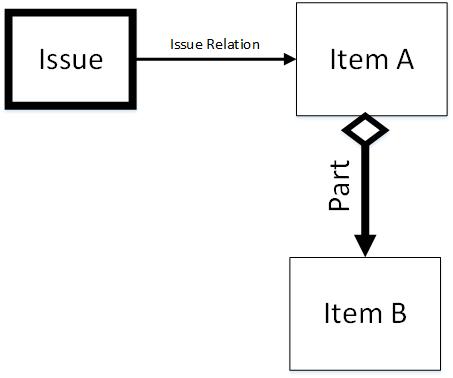
\includegraphics[width=2in]{pdf/blackwhiteipi.png}
%\DeclareGraphicsExtensions{.pdf}
\caption{An overview of the artifacts in SystemWeaver}
\label{fig:ipiov}
\end{figure}

\section{Design of SpeechWeaver}
\label{sec:design}
The architecture of the system that was developed during this research project, SpeechWeaver, consists of a client(s) and a server (see Figure \ref{fig:sysov}). 
The client is a smartphone application frontend, developed in Java for the Android platform, which facilitates user interaction with SpeechServer. 
%Furthermore the client is the GUI that interacts between the user-input and the SpeechServer. 
%Between the client and the SpeechServer a connection is established by TCP/IP and sends strings captured through the speech recognizer on the smart device. 
During usage of the application, text strings are first captured using the speech recognizer in the client which are then sent to SpeechServer using a custom TCP/IP protocol which is described below.

\begin{figure}[!t]

\centering
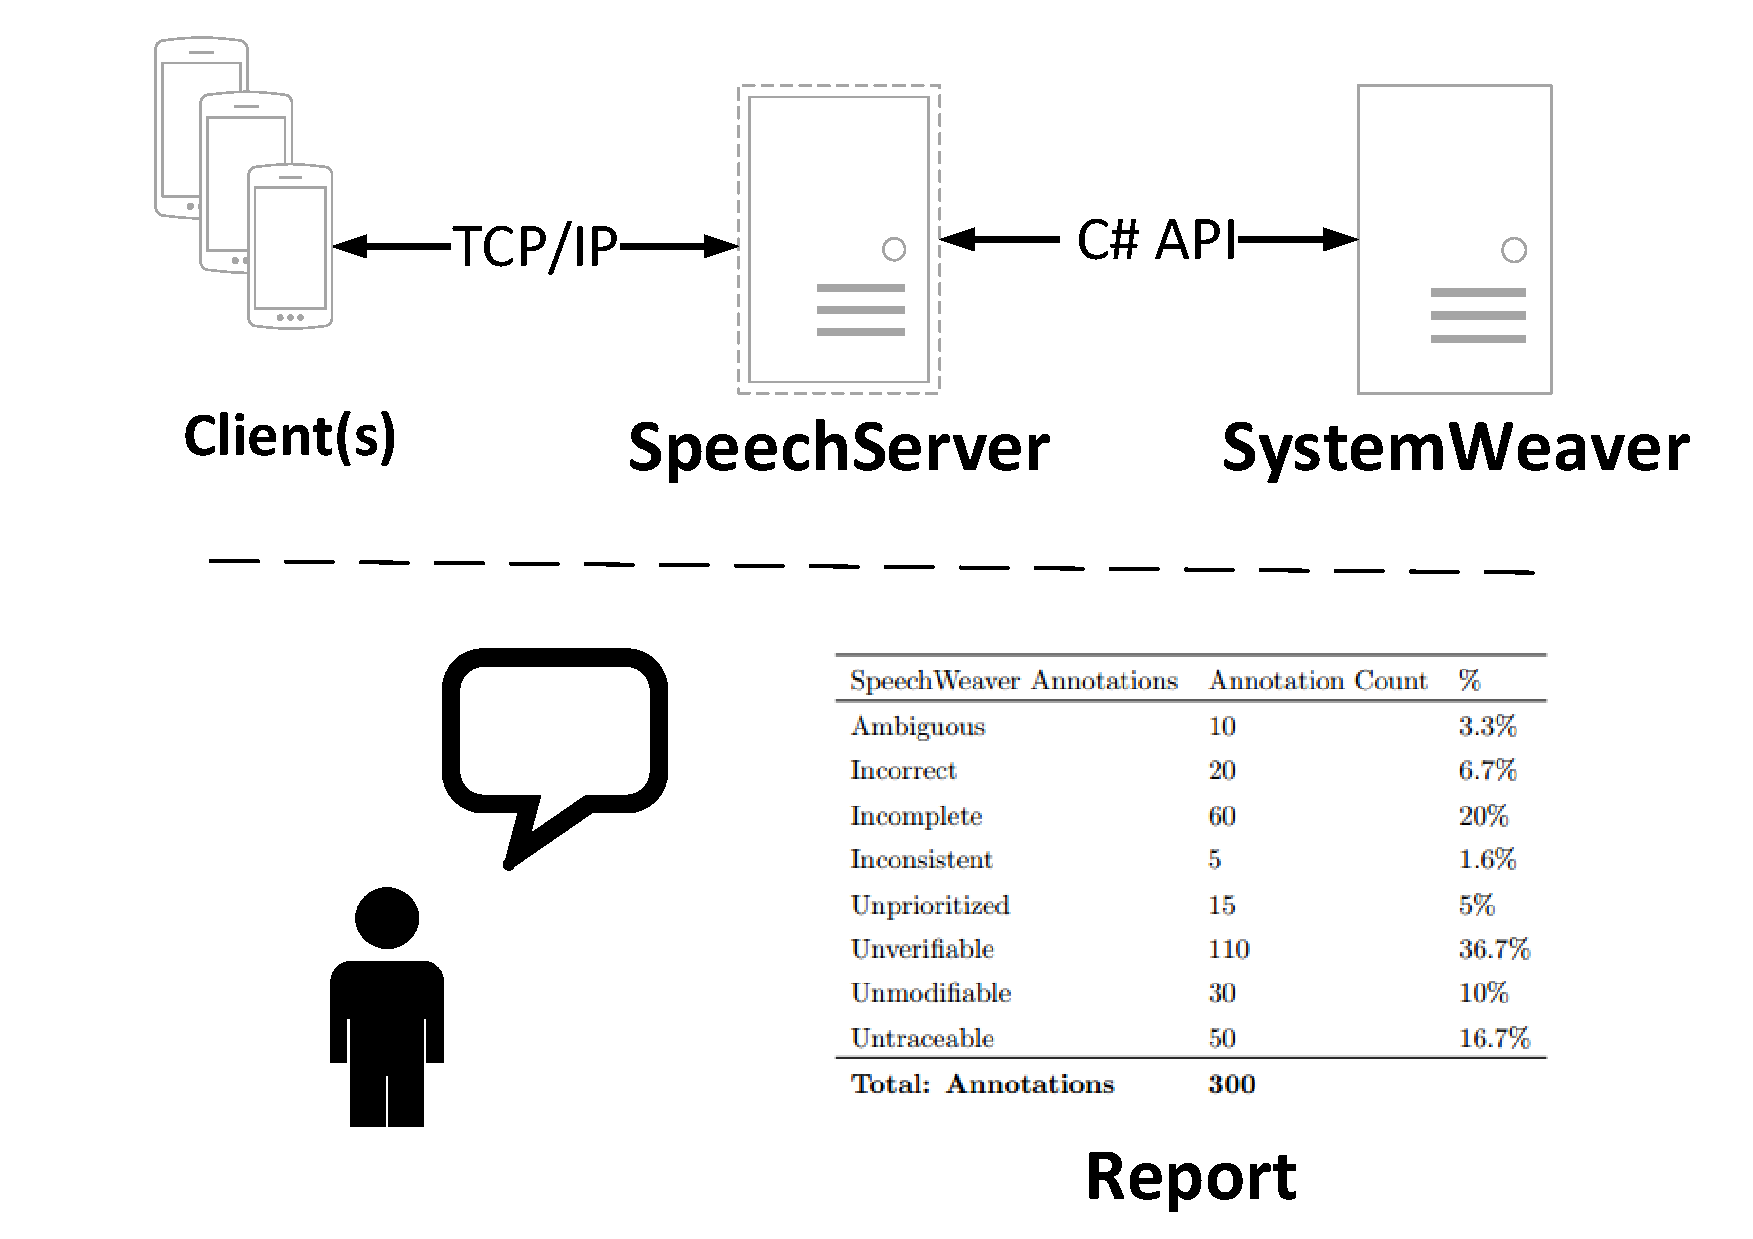
\includegraphics[width=3.5in]{pdf/systemov.pdf}
%\DeclareGraphicsExtensions{.pdf}
\caption{An overview of the SpeechWeaver system}
\label{fig:sysov}
\end{figure}

\subsection{Client}
All user interaction is performed with the client application in SpeechWeaver system, which is developed for Android 4.1 and above to facilitate offline voice typing \cite{offlvoice}.  
%Although this is what is implemented, the type of client is not that important since the communication is done with strings only, so any type of client that can use TCP/IP and send and receive strings can be used. 
However, because of the string based communication, the system does not require an Android based client, only that the client can send and receive TCP/IP messages.
%The use case for different types of clients could be different using their respective advantages, but we have chosen to focus on use cases taking advantage of the mobility provided by smartphones. 
Hence, it is possible to develop clients for different platforms, e.g. desktop applications, in order to take advantage of their respective advantages in different use cases.
However, in this project the focus has been on smartphones in order to take advantage of the mobility that they provide.
%From this point client refers to a smart device using Android.
Therefore all further references in this article to ``the client''  will refer to the developed Android client.

%Within the application, information that is sent from the server to the client is spoken by the application through Android's text-to-speech engine. 
During usage of SpeechWeaver all user interaction is handled through Android's speech-to-text for input and text-to-speech for output which make them auditory.
Furthermore, since this application is tailored for industrial practitioners, information security was also a requirement for the system.
Hence, before the user can interact with the requirement database, the user is required to type in and send user credentials (username and password) to the SpeechServer.
Once user credentials have been verified, the user is presented with a list of to the user available projects that he/she can select to work with. 
After selection of a project, the user can perform three types of actions, which are: 

%\begin{enumerate}
%\item Annotate a requirement - By tapping a button and provide the server with a requirement ID and then an annotation (through their speech)
%\item Annotating a requirement with extra data - By selecting a file from the smart device (e.g. a picture or a recorded sound file) and after that proceeding with the actions mentioned in 1. After those actions are done the application also uploads the file to the SpeechServer.
%\item Generate a report - By tapping a button which triggers the SpeechServer to generate a report over requirements with annotations.
%\end{enumerate}

\begin{enumerate}
    \item Annotate a requirement - Performed by providing the client with a requirement ID and an annotation through auditory input.
	\item Annotate a requirement with additional data - Performed by selecting a file from the smartphone (e.g. a picture or a recorded sound file) followed by the acton described in 1. 
	\item Generate a report - Performed through client interaction that triggers the SpeechServer to generate a report over all annotated requirements.
\end{enumerate}
%EA: Consider changing this list into a table with INPUT and OUTPUT. Above only the input is defined and as you can see I have raised the abstraction level of the descriptions a bit. The reason is because this makes the text more general, i.e. applicable to other platforms than android without detremental effects on the descriptions.

%The text-to-speech- and speech-to-text-engine allows for a communication between the application and user where the user does not need to have any focus on the application. 
The use of auditory interaction with SpeechWeaver removes all need for the user to focus on the application.
%However, to start any of the above mentioned actions, the user needs to tap a button on the screen. 
However, to initiate one of the above mentioned actions the user must interact with client through the Smartphone's touchscreen.
%Though to enable the user to not be interrupted from other work, the action \emph{Annotating a requirement} can be triggered from a button on a bluetooth headset.
Action 1, \emph{Annotate a requirement} can however also be initiated through the button on a bluetooth headset.
Thus facilitating concurrent usage of the system during, for instance, requirements review.


The Android application captures the users voice using the built in API for speech recognition \cite{recAPI}.
When launching the speech recognizer, a pop up dialog appears and a sound is generated to inform the user that the speech recognizer is ready to capture input.
%The user can then state/input a desired phrase. 
The speech recognizer will then record the users input until it does not receive any new input for one second, i.e. until the user goes silent after stating the desired phrase. 
This event will cause the pop up dialog to close and a sound is generated to to inform the user that the speech recognizer has caught the input and is processing it. 
When the speech recognizer has processed the input, it returns up to five results. 
These results are based on how confident the recognizer is that the returned result was correct, where the first of the five results is what the recognizer interpreted as the most likely input from the user.
%EA: fill in the <on/with something> part. I assume you use the Levenshtein algorithm?
%The client has caught input through the speech recognizer, all of the returned results are sent to the server.

%Dessa resultat och hur de räknas ut är providade av android och är för oss en blackbox. Levenshtein används i post-processingen av just dessa resultat.

%"These results are based on how confident the recognizer is that the returned result was correct" - detta är tyvärr det enda android erbjuder som förklaring i sitt API och de har inte presenterat något annat, jag ska se om jag kan leta vidare i patent inatt.
All five alternative user input strings are then sent to the SpeecServer for post-processing. %EA: And the database is updated with a new annotation or a report is developed?

%O&VDessa resultat används bara vid annotationer. Beskrivs senare i serverdelen, bör vi uppdatera med reffar på något sätt? Vi har inte mycket bra underkapitel här...

Android's standard speech recognizer supports different languages. 
However, through out this project, English US was selected used as the primary input language, meaning that the domain of possible interpretations for the speech recognizer were words from the american english dictionary. 
In addition to this dictionary, the speech recognizer also provides the commands "period", "comma", "exclamation mark/point" and "question mark" which are translated into their corresponding characters \cite{typetextbyspeaking}.


%CONTINUE HERE
The communication between SpeechServer and the clients is handled by a custom protocol built on tags that represent different states in the communication. 
The tags are sent over a TCP/IP-socket and are interpreted at the receiving end.
The tags attached to the messages are dependent on which state the system currently is in, i.e. when the client trigger the annotation by sending a requirement title, the messages is tagged with ID (Identification). When the server has found a requirement title (the ID), it returns a message with the tag WFT (Waiting For Tag) and the next output containing the annotation from the client to the server is tagged with ANOT (Annotation). 
%EA: what does dependent on which state the system currently is in mean? Does it mean that the tags change based on the state of client/server? Or does it mean that the tags can only be recieved when the client/server is in a specific state? Clarify and elaborate this a little to give the reader a better understanding of how the tags work and what they represent.

During the setup-phase, after a connection has been established between the client and the server and the user has logged into the system, the server acts as the active part to form a context for the whole system to work within. 
Once the setup-phase is over, SpeechServer takes a passive role where different operations are triggered based on the what is received from the client. % it starts different communication states dependent on what the client send. 
%However, the passive role of the server enabled the communication states to be decided from the client and do not need to be strictly followed if the client decides to abort the current communication-state.
This implementation allows the communication states to be decided from the client and also means that they don't need to be followed if the client decides to abort the current communication state.

Once the setup-phase is over, operations (sending an ID, sending an annotation, create a report etc) are always triggered by the client. The different operations can at any point be aborted and re-selected by the client.
%EA: Not clearly defined above what a communication state actually is. I thought it was the traffic over the socket, but after reading the sentence above I became uncertain. If I can get uncertain, others can as well. Therefore it would be good if you added a sentence or two above that clearly defines what a com. state is.

%O&V Jag ersatte både här och ovan med operations istället. Communication state är en kvarleva från stora rapporten där det fanns en bild. Utökade lite mer.

\subsection{SpeechServer}
The server is written in C\# and runs one thread for each client thereby allowing it to handle multiple clients. 
%EA: Has a good breakdown of items is unintuitive to readers not familiar with SystemWeaver. Can you refine this as: has a good architecture or something more general?
%The SpeechServer handles all clients connecting to the server and listens for input on the predefined socket. 

% O&V var syftningsfel här. Det är inte SystemW som gör att vi kan hantera många klienter på serverns sida utan bara att det är en tråd per client. Tog bort resterande mening
Clients connect to SpeechServer by sending input to a predefined socket that the server listens to.
User authentication, in turn, is handled by checking with SystemWeaver that the provided username and password are both valid.
%EA: The two sentences above confuse me a little. Do you have both a SystemWeaver and SpeechWeaver server in the system? Hasn't been clear from the text but perhaps there is a figure I havn't seen that explains that?

%O&V Finns en bild på detta. Bifogar den i nästa mail och hoppas att den klargör 
As soon as a client connects to the server, the client is given a broker-object by the C\# API to be able to interact with SystemWeaver. 
The broker provides the client with all necessary operations to interact with SystemWeaver, such as authentication, fetching items/parts and writing to SystemWeaver through a connection that is kept alive as long as the client stays connected. 
%This connection is kept alive during the lifetime of the clients connection. 
%The API provides the functionality needed to do the same operations as in the interface of SystemWeaver and some more. REDUNDANT

If the client has not provided a specific project to work on, the server fetches all the projects from the server and sends them to the client and asks which project the user wants to work in. 
The \emph{contexts} from a selected project, which is a delimited part of a project or an abstraction level (e.g. Analysis Level, Design Level, Implementation Level), are treated in the same way by the user, but are traversed to from the project node. 
%EA: A bit ambiguous sentence. Don't quite understand how it works, if you can clarify it that would be good. I however assume that other people might understand it.
%The server sends all context within that project and the user selects one. REDUNDANT
This project retrieval is performed during the \emph{Setup Phase}. %which is accessible from all connection states if the user should choose to change state.

%O&V Tog väck com. states som nu är deprecatat. Det säger inte så där supermycket att man kan välja att köra en setup phase igen, och setup phasen i sig är redan förklarad

After the setup phase, the \emph{Annotation Phase} begins, this is where the user adds an annotation. 
This phase starts with the client providing an input  string with the name of a requirement that the SpeechServer then tries locate. 
When the requirement is found on the server it stores the name temporarily and asks the client what annotation to annotate the requirement with. 
When the annotation has been chosen by the user it is processed and classified into one of the predefined annotations on the server.
The classified annotation is then added to the requirement via the C\#-API of SystemWeaver. 

The server look-up is performed by first asking SystemWeaver for all projects. 
When the user has selected a specific project, the look-up continues by traversing that project to find the project \emph{contexts} (as mentioned above).
After the \emph{context} has been identified, all further look-ups are performed through traversal from that context node. 
This implementation makes the look-up process quite fast since all server data is cached.
The time to perform the look-ups depend on the size of the SRS and the structure of the items the SRS.
%EA: Not sure how the SRS is tied to the database? Missed this connection. Is there a figure or something that explains this?
%EA: Check that above paragraph is correct after the changes I have made

%La till emph på context samt en bakåtreferens (det pratas om vad ett context är i två stycken ovan). Rättade till lite småfel
\subsection{String Processing}
When the server processes the string input it does it in several steps that are dynamic depending on the accuracy of the results. 
%EA: what is name input? This sentence is unclear and because this important to understand the paragraph you should refine it to make it clear what you mean. What is the input? What can it look like? providing an example with actual inputs could help. Example: Using name input, e.g. Ada, as the...
First the client provides the five best results from the speech recognizer (as described above) for an interpreted spoken input. 
%EA: Provides the five best results to what? The user or the server?
%O&V La till att de resultaten kommer från speech reccen, tog väck name input. Ser ingen anledning att den låg där, den refereas inte senare som "name input" någonstans.
First the server tries to find a perfect string match to the five results.
If no perfect matches are found, the Levenshtein distance algorithm is used to find the closest matches on the first of the users input strings. The reason to use all of the five inputs when searching for perfect matches is that the latter results can hold small differences that are crucial for perfect matches, e.g. When a user says``Requirement five", the speech recognizer might interpret the most likely input to be ``requirement five", whilst a latter of the results might  be ``requirement 5". To run all of the five results is an effective way to find more perfect matches, resulting in a better user experience. However, if all five results where run towards the Levenshtein distance algorithm, not enough information would be accessible to say that the closest matches from one of the results from the speech recognizer would be better than another. Therefore, we have chosen to only run the most likely interpreted input against the Levenshtein distance algorithm.
%EA: Only the first out of five strings? Not all five? Clarify.
%O&V: Har försökt att klargöra besluttagandet kring detta. 
Then the server returns the closest matches sorted by their Levenshtein distance from the input string so the user can choose the correct alternative.

There are a few reasons why not to handle the entire input string in one message. 
%EA: correct?
%O&V  correct.
The first reason is that there are problems breaking the input string down in its parts since it's complicated to find which part of the string is the id, and what parts are annotations. 
If the system would have listened for special syntax (example highlighted in bold) such as:
\begin{framed}
\begin{flushleft}
\emph{\textbf{Requirement:} "System should not create a file." \textbf{Annotation: "Ambiguous"}}
\end{flushleft}
\end{framed}

there is a possibility that the requirement could contain these keywords or other syntax words which would result in a faulty delimitation of the string. 
The second reason is that a single string solution requires more from  the user since he/she needs to remember and formulate the syntax, keywords, requirement ID and the annotation before speaking~\cite{memoryCap}. 
Having separated the input into different stages lessens the burden for the system to compensate for these issues, as well as lessen the burden for the user since the user now only needs to answer the questions stated by the application. 
The question-response communication implementation also makes failure mitigation easier if an operation fails since the user can quicker just abort or retry the operation.
%EA: correct?

%O&V: correct.

A way of improving the speech recognizer is to add an algorithm which gives us an indication of what input the user \emph{wanted}, as opposed to what the speech recognizer interpreted. 
When searching for entities within a finite interval, as in the example with requirement names in a requirement database, we improve the searches by measuring an edit-distance between the interpreted input from the speech recognizer and the values in the target domain.
This allows us to narrow down the number of possible results and thereby identify the correct result with higher certainty.
%EA: Last sentence correct?

%O&V: correct.

Edit-distance uses the number of operations needed to transform a string \emph{x} to a string \emph{y}. 
In Levenshtein's string distance function all operations has the same cost, i.e. regardless if you add, delete or modify a character within the string, it is still calculated as a cost of one. 
An edit-distance where this property is fulfilled is often called a Levenshtein distance \cite{blockeel2004}. 

\begin{figure}
\centering
    The distance between two strings \(x,y\) given by \(\operatorname{lev}_{x,y}(|x|,|y|)\) where \\  
    \qquad\operatorname{lev}_{x,y}(i,j) = \begin{cases}
      \max(i,j) &, \min(i,j)=0 \\
      \min \begin{cases}
              \operatorname{lev}_{x,y}(i-1,j) + 1 \\
              \operatorname{lev}_{x,y}(i,j-1) + 1 \\
              \operatorname{lev}_{x,y}(i-1,j-1) + [x_i \neq y_j]
           \end{cases} &, \text{ else}
    \end{cases}
     \caption{The edit-distance (Levenshtein distance) between two strings, \emph{x},\emph{y}, where all operations has a cost of one}
\end{figure}

In our system we use Levenshtein distances when a given input \emph{x} does not have a a requirement name that perfectly matches \emph{x}. 
We then calculate the distance between \emph{x} and all requirements in the given database and returns a set of requirements with the lowest Levenshtein distance, and the user can then chose which requirement the user originally sought.

\subsection{Annotations and Report Generation}
In order to create high quality software requirements specifications (SRS), IEEE have developed a recommended practice for SRSs~\cite{IEEE830}. 
The guideline also defines how to connect the requirements engineering practices to the software lifecycle processes~\cite{IEEE12207}. 
We decided to use the chapter \textit{4.3 Characteristics of a good SRS} from IEEE Recommended Practice for Software Requirements Specifications as the basis for the annotations. 

The provided annotations in SpeechWeaver are the complementary antonyms of the characteristics defined in the IEEE 830 standard. These annotations are just a suggestion of annotations that could be used.
However, they were chosen because they can capture many of the problems a requirement can have. 
This is customizable per customer and organization, to suit problems that a particular organization encounters, this is also customizable in run time and can be changed and perfected continuously during a project to define more narrow definitions of the annotations. 
It is also possible to have synonyms to the annotation tags, so that a user can say \emph{"Not clear."} or \emph{"Not well defined"} instead of \emph{"Ambiguous"}. 
This reduces the burden to remember exact semantics, but the synonyms map to the same tag within the system, that is \emph{Ambiguous}. 

The annotations made by the users are stored in SystemWeaver as individual entities, this allows several users to annotate the same requirement with the same annotation several times. These annotations are stored in an \emph{issue} connected to the requirement, and the connection can be traversed in any direction. The report generation uses these annotations while iterating over the report structure. The output of the report generation are the statistics for the requirements and how many have been annotated with the different annotations. An example can be seen in Figure~\ref{fig:sysov}. Note that in the first table many requirements are tagged with different annotations, this means that if a requirement is annotated several times with the same tag by different users, i.e. several people think that a requirement is \textit{ambiguous}, then the annotation is only counted once for that requirement, to see the status over all requirements. This also means that one requirement can be represented in all categories. In the other table we see the total number of annotations, i.e all annotations are counted.

%EA: you mean the second column right? Or? When defining what table to look at, be very precise. Use the table number, what column to look in, etc.

%\begin{table}[h]
%\centering
%\caption{Example statistics from report generation output, annotated requirements}
%    \begin{tabular}{ l l l}
%        \hline
%        SpeechWeaver Annotations & Annotation Count & \% \\
%        \hline
%        Ambiguous & 5 & 1\% \\ 
%        Incorrect & 10 & 2\%  \\ 
%        Incomplete & 50 & 10\%  \\ 
%        Inconsistent & 1 & 0.2\%  \\
%        Unprioritized & 10 & 2\%  \\
%        Unverifiable & 100 & 20\%  \\
%        Unmodifiable & 20 & 4\%  \\
%        Untraceable & 80 & 16\%  \\ \hline
%        \textbf{Total: Annotated requirements} & \textbf{276} & \\
%        \textbf{Total: Requirements} & \textbf{500} & \\
%        \end{tabular}     
%\label{tab:repgenstat1}
%\end{table}

The generated report also groups annotations by headline so the reader can see all requirements annotated with a specific annotation. 
Furthermore there is headlines for each requirement so the reader can see what problems a particular requirement has. 
The output shows the description for each requirement so the review process becomes as simple as possible. 

The annotations can also be shown for specific time periods or iterations, depending on the project setup. 
This means that statistics can be calculated over time and the data can be plotted to see the history and development of the annotations.


\section{Evaluation}
\label{sec:eval}
The design research project to develop SpeechWeaver was complemented with four evaluation steps as shown in Figure \ref{fig:resov}.
Steps 1 and 2 focused on evaluating to what degree output from speech recognition is useful for identification (step 1) and free-text annotation (step 2) of requirements.
Scaling to realistic requirements database sizes is critical for industrial applicability and since the response time of the system was considered a key characteristic by the company and the identification of requirements dominated the round-trip time, evaluation step 3 measured this time on the server for four different requirement sets.
Finally, step 4 evaluated the SpeechWeaver through a user test and a follow-up interview.
Below we describe the evaluation steps and their results in detail.

%Because an integration between speech recognition software and requirement annotations never had been done before, a design research was carried out. The design research had the main focus on developing a product for annotating SRSs with speech recognition. The research question, methods and contributions of the article can be seen in Figure \ref{fig:resov}. 

%\textbf{The research contained} two experiments to evaluate state of practice speech recognition, an evaluation of the scalability for large scale requirement engineering and a product evaluation containing a user test and a follow-up interview.  

\begin{figure}[!t]
\centering
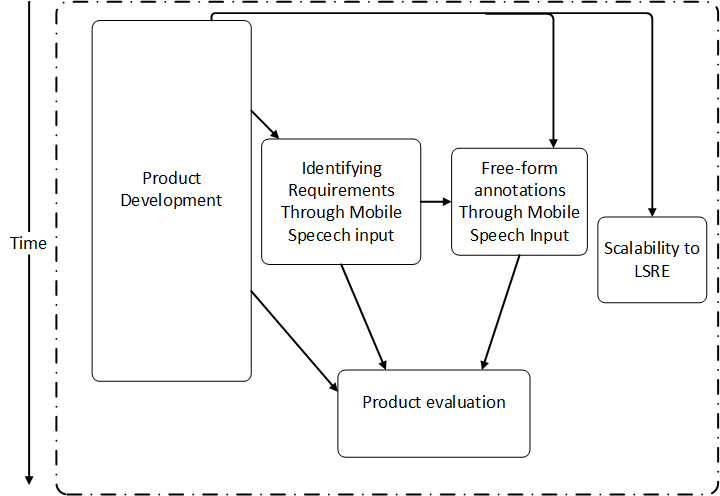
\includegraphics[width=3.5in]{pdf/researchove.png}
%\DeclareGraphicsExtensions{.pdf}
\caption{An overview of the design research}
\label{fig:resov}
\end{figure}

\subsection{Identifying Requirements Through Mobile Speech Input}
%M1

Even though speech recognition algorithms have improved in recent years the error rates can still be high.
This is especially true for the speech recognition available in mobile devices which is typically speaker-independent (which has higher error rates) and has a limited compute power (which makes it impossible to use the best known algorithms).
Our initial results also confirmed that there was often a large discrepancies between the intended requirements supplied as speech input and the output from the speech recognizer.
To make requirements identification possible we extended the system with the Levenshtein string distance as described above.
%When using speech recognizers, there is room for the speech recognition engine to make interpretational errors. A core function in our product was to make up for those errors, something that was done using a string edit distance function when the speech recognizer did not catch the exact sentence that were given through speech. 
To evaluate how well this solution performed an experiment was performed.

The experiment had 10 subjects, all who were students at Chalmers University of Technology, and all with English as their second language. 
Each student was given 10 randomly selected requirement titles from an SRS with 4544 requirements and were asked to speak the titles into the speech recognizer. 
The most likely output from the speech recognizer was then saved and used to evaluate lookup of requirements in that SRS through the Levenshtein edit-distance algorithm.
%The length of the interpreted input and the length of the target requirement title, and the difference between those, were saved for analyzing.
For each input we noted the input length (string length of output from speech recognizer), the target requirement length, distances from input to all requirement titles in the SRS, as well as the rank of the target requirement in the ranking created by the distance function.
An example of the data saved for each input can be found in Table \ref{tab:experimentexample} 

The algorithm was extended to also check for perfect matches (i.e. the interpreted input was exactly the same as the requirement title), and if it was found, the position of the returned result from the speech recognizer were saved. This extension was made to utilize that the speech recognizer returned five different interpretations of the spoken input. If a perfect match was found in any of the five results, the input was never run through the distance function. If a perfect match was not found, only the most likely result from the speech recognizer was run through the distance function. 
%rf: Not clear why you need to extend it to handle perfect input since that would give distance 0!?
%From the Levenshtein edit-distance algorithm, the rank that the originally sought requirement title got out of the 4544 requirements when the interpreted string was given as input was saved, as well as the edit distance between the interpreted string and the originally sought requirement. 

%O&V anledningen till detta är för att i den kunna använda de 5 resultaten returnerade från speechrecen. uppdaterat med "This extension was made to utilize that the speech recognizer returned five different interpretations of the spoken input. If a perfect match was found, the input was never ran through the distance function. If a perfect match was not found, only the most likely result from the speech recognizer was run through the distance function. "


\begin{table}[h]
    \centering
    \caption{Table showing how Levenshtein distance and ranking is calculated for a given input in a closed domain of requirement titles.}
        \begin{tabular}{ | p{2.5cm} | p{2.5cm} | p{1cm} | p{0.5cm} |}
            \hline
            Input & Requirement titles & Distance & Rank\\
            \hline
            And its allies buffet & Initialize buffer & 9 & 1 \\
            \hline
             & Erroneous APLM buffer & 15 & 3 \\
             \hline
             & State monitoring buffer & 14 & 2 \\
             \hline
             & Transaction: Buffer on - Buffer off & 26 & 5 \\ 
             \hline
             & Buffer out of range & 18 & 4 \\ 
             \hline
            \end{tabular}
    \label{tab:experimentexample}
\end{table}
%O&V Uppdateard tabell
%O&V Graf behövs fortfarande, alternativt tabell med frekvens/kumulativ frekevens
To evaluate the performance of our ranking algorithm we consider the lookup a success if the target requirement is ranked among the top five (5) requirements. 
Presenting up to five possible matches to the user was deemed feasible if there is no exact match.
Figure \ref{fig:freqperrank} shows a graph for the percentage of requirements that was ranked among the N top requirements, for increasing numbers of N from 1 to 30.
From the graph we can see that for 73\% of the requirements the target requirement was top ranked and in 93\% of the cases the target rank was among the top five among the 4544 requirements in this SRS.
The mean rank was $6.96$ but this is dominated by a few requirements where the speech recognizer gave output very far from the target requirement; the median rank was 1.

\begin{figure}[!t]

\centering
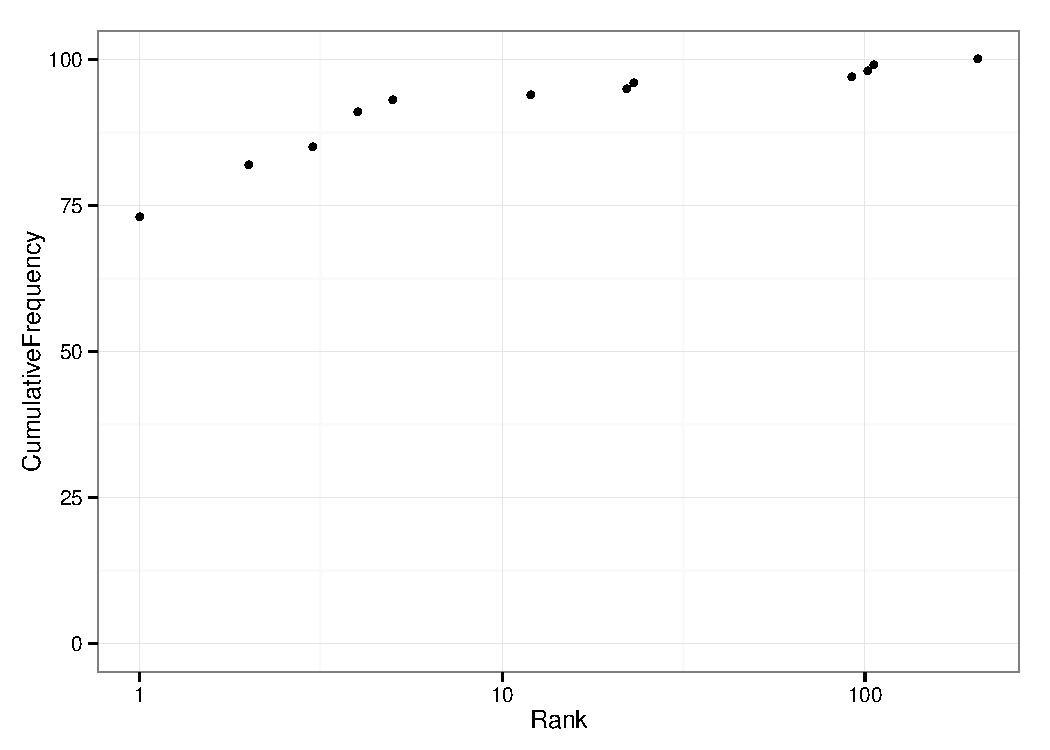
\includegraphics[width=3in]{pdf/freqperrank.pdf}
%\DeclareGraphicsExtensions{.pdf}
\caption{Graph showing the cumulative frequency and the edit distance rank}
\label{fig:freqperrank}
\end{figure}


The speech recognizer delivered 15 perfect matches, and of these 12 where at the first position of the returned results from the speech recognizer. In two of the cases the perfect match was at the speech recognizer's second result, and in one of the cases the perfect match was at the fifth result. In all of the cases, the input to the Levenshtein edit distance algorithm (i.e. the first result returned from the speech recognizer) had the Levenshtein rank 1. The ranges of the inputs that resulted in perfect matches were between 15 to 43 characters, this is most likely because longer strings are more vulnerable to error since any word can be misinterpreted, shorter requirement titles seemed to contain more abbreviations and symbols such as "->" or parentheses/brackets, presumably a consequence of that the recognizer's expected input is words of natural language. None of the given input returned a false perfect match.
%rf: I don't really get the paragraph above. What is the difference between a perfect match and one with a Levenshtein distance of 0? I don't understand why you make a difference.

%O&V: Anledningen är att vi i vår design har valt att kolla om någon av de fem resultat som returneras från Speech Recognizern är en perfekt match. Om så inte är fallet så körs endast det första (most-likely) resultatet mot Levenshtein. Detta eftersom vi i det skedet inte kan avgöra att ett senare resultat är bättre att köra genom levenshtein. I speech-rec-kapitlet pratar vi om att den returnerar fem resultat.

The correlation between Levenshtein distance to the sought requirement title and the difference in length between input and what the speech recognition interpreted can be seen in figure~\ref{fig:levdif}. This figure shows that the Levenshtein distance gives better results for strings with length similar to the target requirement. 
Since the input and interpreted string length often is quite close, this gives good results. 
This also gives a hint that it's better for the user to try to pronounce the whole title, even hard to pronounce symbols and abbreviations, so that the length of the interpreted input is as close to the target requirement as possible, thus making the matching better.
%rf: Förstår inte vad som menas med att uttala abbreviations, kan betyda att säga dem som de står ("U-S-B" tex) eller att "spell them out" dvs beskriva vad de är förkortning för (vilket inte borde vara vad man vill). Klargör.

%O&V: uppdaterat med förklaringen att det är string-längden som är viktig, borde ge läsaren förståelse att man inte är ute efter att "spella them out"

The requirement matching experiment showed that a string edit distance algorithm such as Levenshtein's edit distance can give satisfiable results for matching natural language to name conventions used in an SRS. 
%When the subjects where asked to speak the title of the requirement, and the Levenshtein edit distance algorithm was used towards a SRS of 4544 requirements, 93\% ended up in the rank of one to five. 

\begin{figure}[!t]

\centering
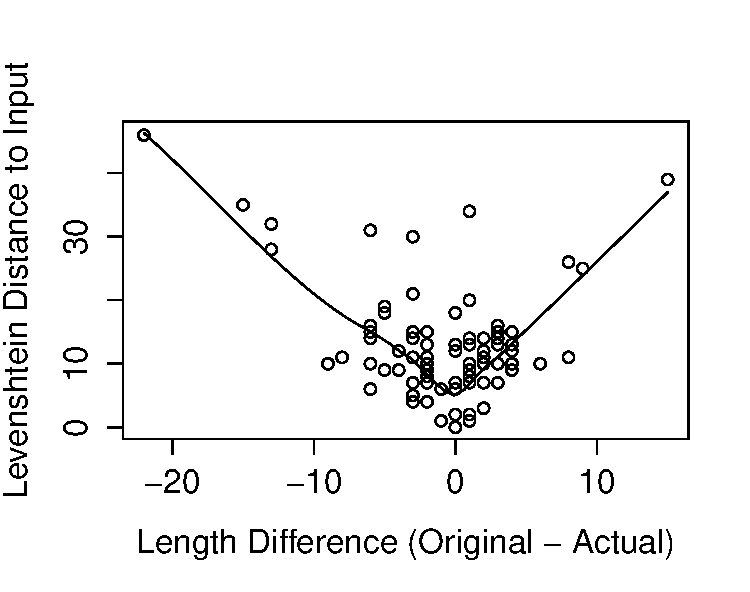
\includegraphics[width=3in]{pdf/Rplot02.pdf}
%\DeclareGraphicsExtensions{.pdf}
\caption{The Levenshtein distance and it's correlation with the difference in input length, the line shows a locally fitted regression}
\label{fig:levdif}
\end{figure}

\subsection{Free-form annotations Through Mobile Speech Input}

Experiment 2 was conducted to evaluate how the speech recognizer behaved with free text input.
Even if this is a typical use of speech recognition we are targetting a specific, technical domain and not everyday speech/text.
Thus, the performance of speech recognition can be expected to be worse.
Since free-form speech recognition would be needed in allowing arbitrary annotations to requirements this is a key concern for our application.

%from a technical domain in a technical domain. 
From the same SRS as mentioned above, 100 sentences were randomly selected. 
The same 10 students as mentioned above were then asked to speak 10 of the sentences into the speech recognizer.
%rf: If it is the same 10 students and 100 requirements it's better to say that.

%O&V säger nu att det vara samma som tidigare nämnts
The best interpreted result from the speech recognizer was then saved in a text file and were later given a value between 0-3, were the numeric defined the level of severeness of the error, as can be seen in Table \ref{tab:severity}

\begin{table}[h!]
    \centering
    \caption{Table showing interpretations of severity}
        \begin{tabular}{ l p{7cm} }
            \hline
            Severity & Meaning \\
            \hline
            0 & No error \\
            1 & Minor error, still comprehensible \\
            2 & Error, hard/impossible to comprehend \\
            3 & Severe Error, meaning of text has changed, but has a viable meaning in the context \\
            \end{tabular}
    \label{tab:severity}
\end{table}

The results from the Recognition Accuracy Experiment in table~\ref{tab:recaccexp} shows that free text speech input is not good enough to provide accurate descriptions as of now. As many as 64\% are not comprehensible, and 10\% can introduce errors if interpreted as written. The number of samples was 98 rather than the stated 100, this was because the experiment equipment failed to record two of the inputs from two different subjects.
\begin{table}[h]
\centering
\caption{Number of descriptions in each severity ranking}
    \begin{tabular}{ l  p{2cm}  p{4cm} }
        \hline
        Severity & Frequency (n=98) & Explanation \\
        \hline
        0 & 8 & No error\\
        1 & 17 &  Minor error, still comprehensible\\
        2 & 63 &  Error, hard/impossible to comprehend\\
        3 & 10 & Severe Error, meaning of text has changed, but has a viable meaning in the context\\
        \end{tabular}
\label{tab:recaccexp}
\end{table}

\subsection{Scalability to large requirements databases}

Software projects in the industry can be very large and complex and often involve several thousand requirements.
To evaluate the scalability of our solution we selected four (4) different requirements databases of medium to large scale from an industrial partner and recorded the execution time for a requirement lookup~\cite{regnell2008}.
All SRS are from the automotive industry and use domain-specific terminology.

% (automotive industry) the industrial partner , a test suite was ran on medium-scaled and large-scaled SRSs  taken from the automotive industry.

%The purpose was to test how the product behaved on different sized software projects, and variables were measured when the product was in action. The variables that were interesting to look at were:

%\begin{itemize}
%\begin{flushleft}
%\item \textbf{SRS size:} number of requirements within the SRS
%\item \textbf{Execution time:} how much time (in milliseconds) it took from the moment the server received the input until it presented %the results to the user. This to evaluate how the system scales in execution time.
%\end{flushleft}
%\end{itemize}

For each of SRSs, a requirement was identified. A user then gave the name of the identified requirement as input to the system through speech. 
Each SRS was queried 30 times and the different values for the above mentioned variables where then saved for analysis.
Since the mobile connection speed as well as latency might vary a lot over time and with the position of the user we measured only the execution time on the server side.
However, this is also realistic since the processing time on the client is minimal and was not considered a factor in user testing.
For this experiment SpeechServer and SystemWeaver is running on a laptop with an dual core Intel i5-350 processor with hyper-threading and 4GB RAM.

%Mean times for the different look-ups are described in table~\ref{tab:timetype} and~\ref{tabl:explsre}. 
%rf: Ändra meningen ovan baserat på att tabellerna nedan tas bort, se kommentarer där. Hänvisa alltså bara till boxplot fig här och ta upp mean time för projekt lookup direkt här. Det är dock lite konstigt med projekt lookup delen eftersom ni bara diskuterar krav här när ni beskriver systemet.
The times shown are from the start of the look-up on the SpeechServer, until the SpeechServer has returned the items and is ready to send to the client. 
Results show that even for large scale requirements engineering the lookup times are manageable. 
%The times in table~\ref{tab:timetype} shows that the number of projects (and contexts within a project) are so low that the times are irrelevant. 
%rf: Meningen ovan behöver slås ihop med den mening som tar upp resultaten för projekt etc.

%O&V: valde att ta väck dessa tider totalt då de inte känns relevanta till undersökningen. Detta är en precondition som görs en gång, utöver detta är dessutom resutlatet att tiderna inte är relevanta för systemet

The time to look up requirements can be seen in Figure~\ref{fig:boxplots}.
%O&V Hur reffar vi dessa på ett bra sätt och har en bra caption på de?
In practice the look up items is sometimes unpredictable since SystemWeaver as well as SpeechServer does caching internally.
Performance can depend on what has been searched before and other factors, such as other users and how much have and can be cached. 
These results we got here are close to what can be expected in actual use (excluding the network latency and speed as discussed above).
The lookup times are dominated not by the ranking through string distance but by the lookup of the requirements in the db.
Since these lookups go through the existing API it was not feasible to propose changes to the underlying system.
For speedier look ups on frequently performed tasks SpeechServer could cache the requirements titles locally.
The maximum observed processing time for the Levenshtein ranking was in the order of 300ms, even for the largest SRS.
Thus, even though many data structures and solutions, such as for example suffix filters~\cite{karkkainen2007faster}, for fast and approximate string matching could be used they are not warranted unless the requirements db's are very large (on the order of 10,000 to 100,000 requirements).


\begin{figure}[!t]
\centering
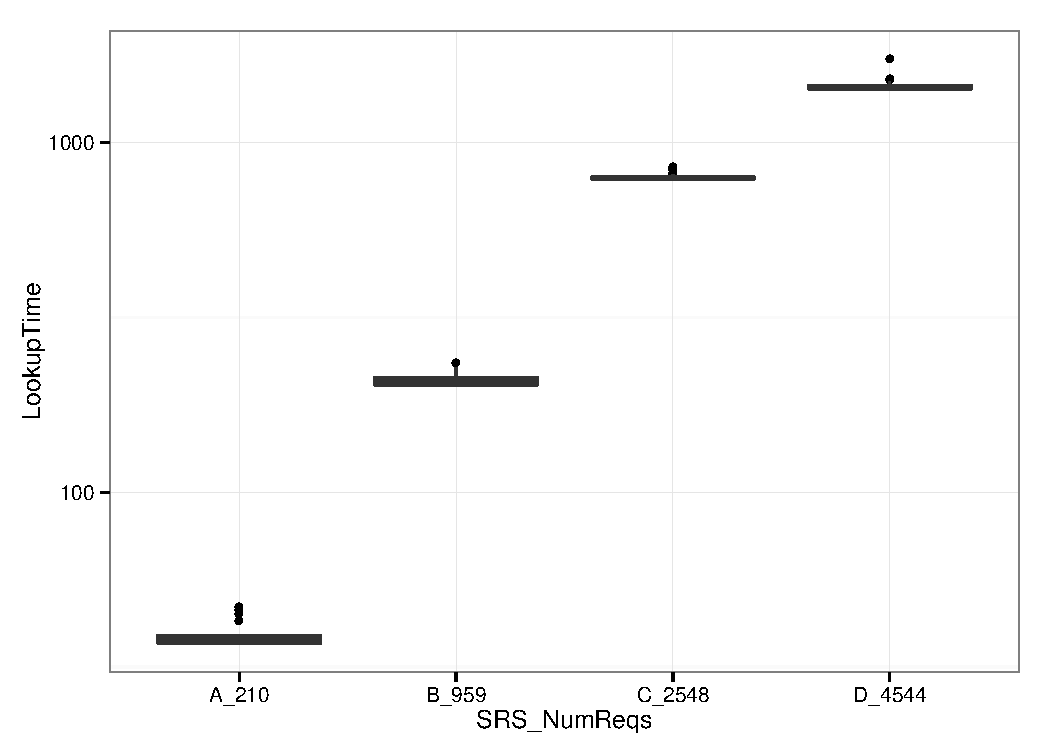
\includegraphics[width=3.5in]{pdf/boxplots.pdf}
%\DeclareGraphicsExtensions{.pdf}
\caption{Time to look up requirements}
\label{fig:boxplots}
\end{figure}



%rf: Lägg in i bib:
% @inproceedings{karkkainen2007faster,
%  title={Faster filters for approximate string matching},
%  author={K{\"a}rkk{\"a}inen, Juha and Na, Joong Chae},
%  booktitle={Proc. ALENEX},
%  volume={7},
%  pages={84--90},
%  year={2007}
%}

%\begin{table}[h]
%\centering
%\caption{Approximate times to look up projects and contexts, mean of 10 runs}
%\centering
%    \begin{tabular}{l l l}
%        \hline
%        Type & Quantity & Time in ms \\
%        \hline
%       Projects & 89 & 2 \\
%        Contexts & 3 & 1 \\
%        \end{tabular}
%\label{tab:timetype}
%\end{table}
%rf: Skippa ovanstående tabell och skriv bara de tiderna i brödtexten ovan istället. För lite information för att motivera en tabell.

%O&V: Tog bort tabell och även brödtext

%\begin{table}[h]
%\centering
%\caption{Times to look up item requirements, mean of 31 runs}
%\centering
%    \begin{tabular}{l  l}
%        \hline
%        Requirements & Time in ms \\
%        \hline
%        4544 & 1450 \\
%        959 & 39 \\
%        210 & 209 \\
%        2548 & 797
%        \end{tabular}
%\label{tabl:explsre}
%\end{table}
%rf: Byt ut ovanstående tabell mot boxplot. Använd antal krav som "label" på x axeln och tid (i ms) som skala på y axeln.
%O&V Boxplottar tillagda. Hur skall dessa referreras i texten? 

\subsection{User testing and interviews}

The end user evaluation of SpeechWeaver contained two parts, monitored user tests followed by interviews. 
The subjects for the user test was five requirement- and application-engineers at Systemite AB.

The subjects was given a short introduction about the features and the design of the application and was then given five randomly selected requirements within a chosen context, and was asked to create an issue to each of the requirement with the application. Out of these five, two of the issues required an attached file. After the requirements were annotated the user sat down and explored the result of the actions by looking at the updates that had been added in SystemWeaver. 

Finally the user was interviewed about the experience of using the application. The main focus of the interview was the experience of using speech as input, but also overall impressions of the usability and ease of use of the product as a whole. 

Below we present results from this interview in two parts, (1) the annotations and the usefulness of those, and (2) the overall experience of the application.
%rf: Beskrivningen ovan upprepar sig något. Försök förenkla språket.
%O&V: Uppdaterat 
All of the interviewed subjects used TODO-lists in the format of analog or digital notes to their ongoing projects. What they found to be a huge profit with the annotations on the requirements was that there were a direct connection between the TODO-entity (the annotation) and the actual requirement. 

A factor that arose as very important for all of the interviewees were the content of the annotations. They found it very important that the naming of the annotations fitted the way they worked with maintenance of projects, and that there needed to be a clear definition and distinction between each and one of the annotations. The interviewees expressed that the annotations without any more descriptive information (a file or a description field) were better for peer-reviewing purposes (i.e. letting users go through the SRS and go through the annotations in a group format), where as an annotation that contained descriptive information were better for actual modifications and improvements on the requirement. 

The key notes that the subjects expressed as very positive was the accuracy and the response time of the application. 

Many subjects expressed the usefulness of the mobility in the application. To be able to query an SRS with several thousand of requirements anywhere, from the car or the bar, was considered a huge advantage. The solution was also considered very light weight, and the flow combined with the low amount of time to create an issue were expressed as an easy solution to directly ventilate their thoughts towards the SRS, instead of a tidy operation when they would otherwise have to make several operations to navigate and interact with SystemWeaver.

Some felt uncomfortable using speech as the main input for the application. Moreover, requirement titles that contained "special" characters (e.g. "\#", "-\textgreater", "=") or abbreviations were found hard to translate to spoken words. Another problem that was pointed out was the sound that was produced during the operation, and several of the subjects stated that they would not use it in an office environment.

%rf: Ni får gärna skriva lite mer om resultaten av user testing om ni har något.
%O&V Har inget mer att presentera som framkom i intervjuerna, skulle bara vara "ordbajs"/utvecklingarna om samma saker
\section{Discussion}
\label{sec:disc}
Speech recognition have developed over the years, but as shown by our results, it is still not good enough to recognize longer, natural language free form sentences.
This limits the range of maintenance actions for which our system can be used.
For example, we cannot allow the substitution of longer sequences of text, such as in requirements descriptions or rationales often found in specifications.

With the use of simple string distance measures and by constraining the set of sentences being matched against the output from the speech recognizer can be used to query, and thus annotate, text entities, such as requirements, even in large software development projects.
In our experiment the constrained set was all the requirement titles of the specification.
But future work could consider other constraining sets.
For example, once a requirement has been selected for edits, which attribute of it, and potentially which sentence within the value of an attribute, to change or annotate could be found through a similar use of constrained string distance matching.
Thus we consider our results an important first step towards a more extensive requirements annotation and maintenance system.

Our results and user testing also show that mobile devices enables speech recognition as a tool for querying requirement specifications, and that this opens up new possibilities for when and where you can `reach' the specifications. 
This increased accessibility together with the ease of use that the users expressed when testing the system could lead to a change in how software engineers view maintenance tasks.
Today it is often considered a disturbance and chore and as being troublesome.

To annotate SRS could possibly be used in a similar manner to how defect inflow can be predicted as described by \citet{mstaronmetrics}. This would allow for requirement engineers and other people associated to the software documentation to prepare and revise their work with the quality of the SRS.

A threat to the validity of this research is that only five requirements engineers was used in the user testing and that they were all from the same company. 
However, since they work with a software development and requirements support tool and also work with customers they have a broad experience from many different software development contexts.
Another threat to the generalizability of our results is that all four requirements specifications used in the experiments was from one and the same company, in the automotive domain.
Since our system is not adapted in any way to the specific domain or vocabulary used in these specifications we do not consider this a major threat.
In our data collection and experiments we have used randomization and replicate measurements to avoid threats to internal and conclusion validity.
%rf: Jag skriver detta när jag ser hur mycket plats det finns kvar. Inte säkert vi har plats för så mycket mer...
% An example of a floating figure using the graphicx package.
% Note that \label must occur AFTER (or within) \caption.
% For figures, \caption should occur after the \includegraphics.
% Note that IEEEtran v1.7 and later has special internal code that
% is designed to preserve the operation of \label within \caption
% even when the captionsoff option is in effect. However, because
% of issues like this, it may be the safest practice to put all your
% \label just after \caption rather than within \caption{}.
%
% Reminder: the "draftcls" or "draftclsnofoot", not "draft", class
% option should be used if it is desired that the figures are to be
% displayed while in draft mode.
%
%\begin{figure}[!t]
%\centering
%\includegraphics[width=2.5in]{myfigure}
% where an .eps filename suffix will be assumed under latex, 
% and a .pdf suffix will be assumed for pdflatex; or what has been declared
% via \DeclareGraphicsExtensions.
%\caption{Simulation Results.}
%\label{fig_sim}
%\end{figure}

% Note that IEEE typically puts floats only at the top, even when this
% results in a large percentage of a column being occupied by floats.


% An example of a double column floating figure using two subfigures.
% (The subfig.sty package must be loaded for this to work.)
% The subfigure \label commands are set within each subfloat command,
% and the \label for the overall figure must come after \caption.
% \hfil is used as a separator to get equal spacing.
% Watch out that the combined width of all the subfigures on a 
% line do not exceed the text width or a line break will occur.
%
%\begin{figure*}[!t]
%\centering
%\subfloat[Case I]{\includegraphics[width=2.5in]{box}%
%\label{fig_first_case}}
%\hfil
%\subfloat[Case II]{\includegraphics[width=2.5in]{box}%
%\label{fig_second_case}}
%\caption{Simulation results.}
%\label{fig_sim}
%\end{figure*}
%
% Note that often IEEE papers with subfigures do not employ subfigure
% captions (using the optional argument to \subfloat[]), but instead will
% reference/describe all of them (a), (b), etc., within the main caption.


% An example of a floating table. Note that, for IEEE style tables, the 
% \caption command should come BEFORE the table. Table text will default to
% \footnotesize as IEEE normally uses this smaller font for tables.
% The \label must come after \caption as always.
%
%\begin{table}[!t]
%% increase table row spacing, adjust to taste
%\renewcommand{\arraystretch}{1.3}
% if using array.sty, it might be a good idea to tweak the value of
% \extrarowheight as needed to properly center the text within the cells
%\caption{An Example of a Table}
%\label{table_example}
%\centering
%% Some packages, such as MDW tools, offer better commands for making tables
%% than the plain LaTeX2e tabular which is used here.
%\begin{tabular}{|c||c|}
%\hline
%One & Two\\
%\hline
%Three & Four\\
%\hline
%\end{tabular}
%\end{table}


% Note that IEEE does not put floats in the very first column - or typically
% anywhere on the first page for that matter. Also, in-text middle ("here")
% positioning is not used. Most IEEE journals/conferences use top floats
% exclusively. Note that, LaTeX2e, unlike IEEE journals/conferences, places
% footnotes above bottom floats. This can be corrected via the \fnbelowfloat
% command of the stfloats package.



\section{Conclusion}
\label{sec:concl}
This paper presents the design, implementation and evaluation of a lightweight system for annotating requirements specifications. 
By connecting the default speech recognition available in a present-day (Android-based) mobile device to a commercial software development management tool, we can allow access and annotation of large-scale requirements databases from anywhere where you can reach the Internet. 

Speech recognition has improved considerably in recent years and its accuracy has increased. 
However, one of our experiments show that the accuracy of speech recognition available in mobile devices today is not yet adequate to allow free text input, such as comments or larger edits, in the often specialized-vocabulary, technical domains of industrial requirements specifications (SRSs). 
Even when used for shorter inputs, such as the lookup of a requirement prior to annotating it, accuracy is often poor. 
By extending our system with a simple string distance measurement we could improve accuracy considerably for the more limited lookup and annotation tasks.
With the off-the-shelf speech recognizer and input from 10 non-native English speaking test subjects (with English as their second language) the system ranked the targeted requirement among the top five requirements returned 93\% of the time for 98 requirements randomly sampled from a SRS containing 4544 requirements.

%an experiment using a speech recognizer built upon a natural language to evaluate towards a technical domain such as a software requirement specification showed that state-of-the-art speech recognition is yet inadequate when free text is allowed. When using string edit distance algorithms such as Levenshtein's edit distance-algorithm can improve the deficiency in the speech recognizer's accuracy when using it towards a closed domain, such as one sentence titles for entities, even when the titles are built upon a technical language. When using an off-the-shelf speech recognizer with English US as the natural language base, and test subjects with English as their second language, the edit distance-algorithm provided the sought entities in a top five result (ranked on the distance between the interpreted input from the speech recognizer and the sought entity) out of 4544 of entities in 93\% of the cases.

Moreover, a scalability experiment showed that with a mobile device, you can query and work with large scale SRSs with feasible round-trip times. 
Results from the database lookups were presented to the users within seconds even for SRSs with several thousand requirements.
Together with speech recognizers within mobile smart devices this enables users to reach and query large scale requirement databases anytime, anywhere.

In user testing with five requirement engineers and managers at our industrial collaborator the system was considered surprisingly 
accurate and responsive.
The users considered the system a suitable addition to their workflow, in particular as a substitute for their present day lists of requirements to change and updates to be made.
They also noted that the system was useful in requirements reviews.
For more extensive maintenance work it would need to allow longer input of more free form text.
Some users also was concerned about the noise they would generate while using the application; they said they would be reluctant to use it in an open office layout.

Annotations on `softer' software engineering artifacts, such as requirements, is an unexplored area. 
We have presented a way to use these annotations as a lightweight maintenance- and peer-review tool for marking requirements during development and maintenance of large-scale industrial requirements specifications. 
Future research should investigate the long-term effects of such annotations on the quality and efficiency of requirements evolution and maintenance.
Our system can also be used to collect metrics on requirements churn, quality and change frequencies.
To improve speech recognition accuracy future research could build up a specific speech recognition locales and dictionaries specific to the technical terms commonly seen in the technical areas related to software engineering and development.

%For future research, we suggest that the implemented system should be carried out in a long term software project to evaluate the impact of annotations on softer artifacts. The statistics and metrics that were produced presents possible areas of research such as inflow prediction and more background on when quality issues are introduced in SRSs. Another research could be to implement a speech recognition locale built up on technical terms to improve the accuracy of the system.

% conference papers do not normally have an appendix


% use section* for acknowledgement
\section*{Acknowledgment}

The authors would like to thank Systemite AB for their cooperation during this research. 

%\hfill O. Petersson, V. Mellgren, R. Feldt, E. Alegroth
 
%\hfill May 13, 2013



% trigger a \newpage just before the given reference
% number - used to balance the columns on the last page
% adjust value as needed - may need to be readjusted if
% the document is modified later
%\IEEEtriggeratref{8}
% The "triggered" command can be changed if desired:
%\IEEEtriggercmd{\enlargethispage{-5in}}

% references section

% can use a bibliography generated by BibTeX as a .bbl file
% BibTeX documentation can be easily obtained at:
% http://www.ctan.org/tex-archive/biblio/bibtex/contrib/doc/
% The IEEEtran BibTeX style support page is at:
% http://www.michaelshell.org/tex/ieeetran/bibtex/
%\bibliographystyle{IEEEtran}
% argument is your BibTeX string definitions and bibliography database(s)
%\bibliography{IEEEabrv,../bib/paper}
%
% <OR> manually copy in the resultant .bbl file
% set second argument of \begin to the number of references
% (used to reserve space for the reference number labels box)

\bibliographystyle{IEEEtran}
\bibliography{IEEEabrv,references}

%\begin{thebibliography}{1}

%\bibitem{IEEEhowto:kopka}
%H.~Kopka and P.~W. Daly, \emph{A Guide to \LaTeX}, 3rd~ed.\hskip 1em plus
%  0.5em minus 0.4em\relax Harlow, England: Addison-Wesley, 1999.

%\end{thebibliography}


% that's all folks
\end{document}








